%%%%%%%%%%%%%%%%%%%%%%%%%%%%%%%%%%%%%%%%%
% a0poster Portrait Poster
% LaTeX Template
% Version 1.0 (22/06/13)
%
% The a0poster class was created by:
% Gerlinde Kettl and Matthias Weiser (tex@kettl.de)
% 
% This template has been downloaded from:
% http://www.LaTeXTemplates.com
%
% License:
% CC BY-NC-SA 3.0 (http://creativecommons.org/licenses/by-nc-sa/3.0/)
%
%%%%%%%%%%%%%%%%%%%%%%%%%%%%%%%%%%%%%%%%%

%----------------------------------------------------------------------------------------
%	PACKAGES AND OTHER DOCUMENT CONFIGURATIONS
%----------------------------------------------------------------------------------------

\documentclass[a0,portrait]{a0poster}
\usepackage[utf8]{inputenc}   %%% JTO
\usepackage[francais]{babel} %%% JTO

\usepackage{multicol} % This is so we can have multiple columns of text side-by-side
\columnsep=100pt % This is the amount of white space between the columns in the poster
\columnseprule=3pt % This is the thickness of the black line between the columns in the poster

\usepackage[svgnames]{xcolor} % Specify colors by their 'svgnames', for a full list of all colors available see here: http://www.latextemplates.com/svgnames-colors

\usepackage{times} % Use the times font

\usepackage{graphicx} % Required for including images
\graphicspath{{figures/}} % Location of the graphics files
\usepackage{booktabs} % Top and bottom rules for table
\usepackage[font=normalsize,labelfont=bf]{caption} % Required for specifying captions to tables and figures
\usepackage{amsfonts, amsmath, amsthm, amssymb} % For math fonts, symbols and environments
\usepackage{wrapfig} % Allows wrapping text around tables and figures
\usepackage{tikz}
\usetikzlibrary{calc,trees,positioning,arrows,chains,shapes.geometric,%
decorations.pathreplacing,decorations.pathmorphing,shapes,%
matrix,shapes.symbols,plotmarks,decorations.markings,shadows}
\usepackage{array}
\renewcommand\familydefault{cmss}

\newcommand{\captioncolor}{\color{black}}

\begin{document}

%----------------------------------------------------------------------------------------
%	POSTER HEADER 
%----------------------------------------------------------------------------------------

% The header is divided into two boxes:
% The first is 75% wide and houses the title, subtitle, names, university/organization and contact information
% The second is 25% wide and houses a logo for your university/organization or a photo of you
% The widths of these boxes can be easily edited to accommodate your content as you see fit

\begin{minipage}[b]{0.75\linewidth}
\veryHuge \color{NavyBlue} \textbf{Stage de Recherche en Informatique (Sup\'e{}lec 2A)} \color{Black}\\ % Title
\Huge\textit{Fixed-parameter tractability of counting small minimum (S,T)-cuts }\\[18mm] % Subtitle
\huge \textbf{Benjamin MOUSCADET}\\[0.5cm] % Author(s)
\huge LRI, CentraleSupélec, Université Paris-Saclay\\[0.4cm] % University/organization
\end{minipage}
%
\begin{minipage}[b]{0.25\linewidth}

\includegraphics[width=15cm]{logo_lri.jpg}\\
\end{minipage}

\vspace{1cm} % A bit of extra whitespace between the header and poster content

%----------------------------------------------------------------------------------------

\begin{multicols}{2} % This is how many columns your poster will be broken into, a portrait poster is generally split into 2 columns

%----------------------------------------------------------------------------------------
%	CONTEXTE
%----------------------------------------------------------------------------------------

\section*{Contexte du stage}

Il s'agissait d'un stage de deuxième année au Laboratoire de Recherche en Informatique, sous la direction du Pr. Joanna Tomasik. Si la plupart des stages se font en entreprise, j'ai préféré effectuer un stage de recherche, continuant mon apprentissage en recherche initié lors du projet long. J'ai travaillé pendant deux mois avec Pierre Bergé, doctorant, sur un des problèmes qu'il traite dans sa thèse. J'ai également participé à la rédaction d'une publication scientifique, issue du problème abordé.


%----------------------------------------------------------------------------------------
%	STAGE DE RECHERCHE
%----------------------------------------------------------------------------------------

\color{NavyBlue}

\section*{Pourquoi faire un stage de recherche ?}

\begin{enumerate}
\item La recherche est un monde complètement différent, avec lequel les étudiants ne sont que peu familiarisés
\item Les opportunités de faire de la recherche en école d'ingénieur ne sont pas si nombreuses, mais permettent de se faire une idée plus précise de ce qui est attendu d'un chercheur, ou d'un doctorant
\item La recherche confronte chacun avec ses propres capacités, les seules limites sont celles de l'imagination et la rigueur du chercheur. C'est un travail en autonomie
\item La recherche est un monde intellectuellement très stimulant, et donne la possibilité de résoudre des problèmes sans limite de difficulté
\item Un stage de recherche permet de comprendre mieux le système des publications auquel sont soumis tous les chercheurs
\item Les doctorants sont une population jeune et dynamique avec qui échanger est très stimulant, chacun offrant un point de vue unique sur son domaine d'expertise

\end{enumerate}

%----------------------------------------------------------------------------------------
%	POSITION DU PROBLÈME
%----------------------------------------------------------------------------------------

\color{Black}

\section*{Définition du problème}

Donnés un graphe $G=(V,E)$ et deux ensembles $S,T \subseteq V$ de sommets de $G$, on définit :
\begin{itemize}
  \item une \textit{cut} $X \subseteq E$ est un ensemble d'arêtes du graphe telle qu'il n'existe aucun chemin reliant $S$ à $T$ dans le graphe $G$ privé de $X$
  \item une \textit{mincut} est une cut (non nécessairement unique) dont le nombre d'arêtes est minimun
\end{itemize}
Dans ce problème, on cherche un algorithme qui \textbf{compte toutes les \textit{mincuts}} du graphe.

\begin{center}\vspace{1cm}
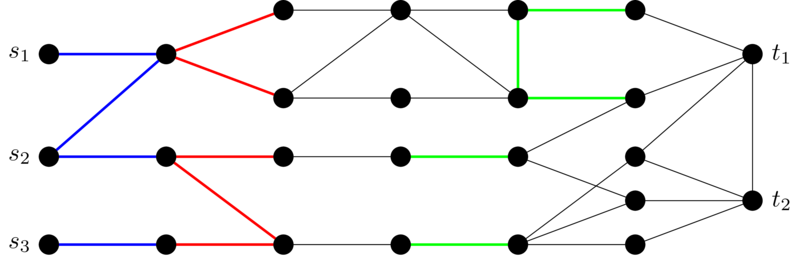
\includegraphics[width=0.90\linewidth]{min-cut}
\captionof{figure}{\captioncolor Deux exemples de cuts (en rouge et vert, taille 5) et une mincut (en bleu, taille 4)}
\end{center}\vspace{8mm}

%----------------------------------------------------------------------------------------
%	COMPLEXITÉ
%----------------------------------------------------------------------------------------

\section*{Complexité du problème}

\begin{itemize}
  \item Trouver la taille des \textit{mincuts} est un problème \textbf{P} : cela peut être fait en temps polynomial $\mathcal{O}(n m^2)$ où $n = |V|$ est le nombre de sommets du graphe et $m = |E|$ es le nombre de ses arêtes
  \item En revanche compter le nombre total de \textit{mincuts} est un problème \textbf{NP-HARD} : il n'existe pas d'algorithme polynomial pour le faire 
\end{itemize}

\begin{center}\vspace{1cm}
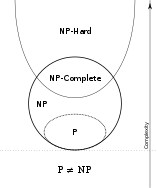
\includegraphics[width=0.35\linewidth]{PNP}
\captionof{figure}{\captioncolor Les différentes classes de complexité de problèmes}
\end{center}\vspace{8mm}

Alors que la solution exacte d'un problème \textbf{P} peut être obtenue en temps raisonnable sur des instances de grande taille ($n=10^4$ par exemple), la résolution d'un problème \textbf{NP-HARD} nécessitera généralement un temps exponentiel en la taille de l'instance. \vspace{5mm}
  
\newcommand{\asize}{\large}
\newcommand{\cc}{\color{red}}
\begin{center}

 \begin{tabular}{>{\asize}c|>{\asize}c|>{\asize}r|>{\asize}r|>{\asize}r|>{\asize}r|>{\asize}r|>{\asize}r}
  \centering
     Complexité & Dénomination & \multicolumn{1}{|c|}{$n=5$} & \multicolumn{1}{c|}{$n=10$} & \multicolumn{1}{c|}{$n=50$} & $n=1000$ & $n=10000$ & $n=1 000 000$ \\
    \midrule
    $\mathcal{O}(\log(n))$ & \cc Logarithmique & $10$ ns & $10$ ns & $20$ ns & $30$ ns & $40$ ns & $60$ ns \\
    $\mathcal{O}(n)$      & \cc Linéaire      & $50$ ns & $100$ ns & $500$ ns & $10\ \mu$s & $100\ \mu$s & $10$ ms \\ 
    $\mathcal{O}(n^2)$    & \cc Quadratique   & $250$ ns& $1\ \mu$s & $25\ \mu$s &$10$ ms & $1s$ & $2.8$ h \\ 
    $\mathcal{O}(n^3)$    & \cc Cubique       & $1.25\ \mu$s & $10\ \mu$s & $1.25$ ms & $10$ s  & $2.7$ h & $316$ ans \\
    $\mathcal{O}(2^n)$    & Exponentielle & $320$ ns & $10\ \mu$s & $130$ jours & $10^{59}$ ans & --- & --- \\
    $\mathcal{O}(n!)$     & Factorielle    & $1.2\ \mu$s & $36$ ms & $10^{48}$ ans & --- & --- & --- \\
  \end{tabular}
  

%  \begin{tabular}{>{\asize}c|>{\asize}c|>{\asize}c|>{\asize}c|>{\asize}c|>{\asize}c|>{\asize}c|>{\asize}c}
%  \centering
%     Complexité & Dénomination & $n=5$ & $n=10$ & $n=50$ & $n=1000$ & $n=10000$ & $n=1 000 000$ \\
%    \midrule
%    \cc$O(log(n))$ & \cc Logarithmique & $10$ns & $10$ns & $20$ns & $30$ns & $40$ns & $60$ns \\
%    \cc$O(n)$      & \cc Linéaire      & $50$ns & $100$ns & $500$ns & $10mu s$ & $100\mu s$ & $10ms$ \\ 
%    \cc$O(n^2)$    & \cc Quadratique   & $250ns$& $1\mu s$& $25\mu s$&$10ms$ & $1s$ & $2.8h$ \\ 
%    \cc$O(n^3)$    & \cc Cubique       & $1.25\mu s$ & $10\mu s$ & $1.25ms$ & $10s$ & $2.7h$ & $316$ ans \\
%    $O(2^n)$    & Exponentielle & $320ns$ & $10\mu s$ & $130$ jours & $10^{59}$ans & --- & --- \\
%    $O(n!)$     & Factorielle    & $1.2 \mu s$ & $36 ms$ & $10^{48}$ans & --- & --- & --- \\
%  \end{tabular}
  
  
  \captionof{table}{\captioncolor Temps de calcul pour différentes complexités, à $10^8$ flops (opérations/seconde). En rouge les complexités polynomiales ou sub-polynomiales} 
\end{center}\vspace{8mm}

%----------------------------------------------------------------------------------------
%	Complexité FPT
%----------------------------------------------------------------------------------------

\section*{Approches possibles}

  \begin{enumerate}
    \item \textbf{Algorithmes d'approximation} : une solution approchée en temps polynomial
    \item \textbf{Algorithmes exacts mais polynomiaux pour certaines instances du problème seulement} 
  \end{enumerate}


\begin{center}%%%%\vspace{1cm}
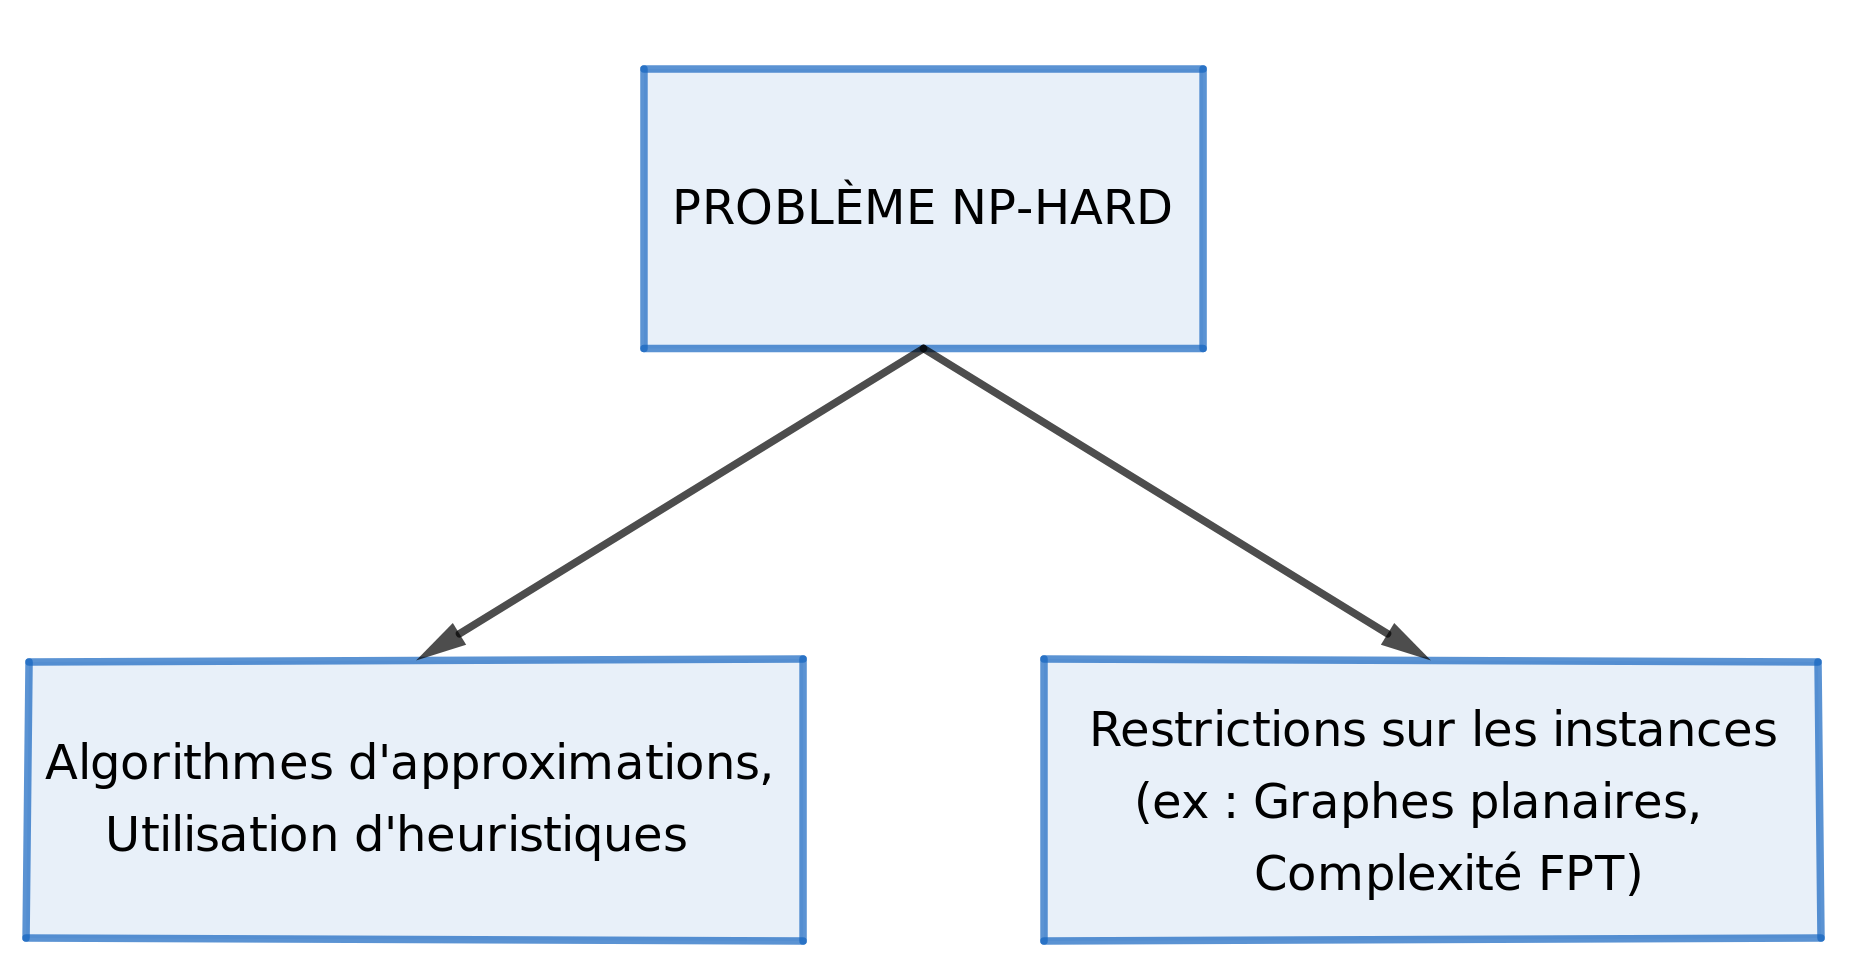
\includegraphics[width=0.55\linewidth]{solutions}
%%%\captionof{figure}{\captioncolor Plusieurs solutions possibles lorsqu'on est confrontés à un problème NP-HARD}
\end{center}\vspace{1cm}


\begin{itemize}
  \item On choisit de travailler sur les instances dont la taille $p$ de la \textit{mincut} est petite : des termes exponentiels en $p$ dans la complexité sont autorisés
  \item  La \textbf{complexité FPT} s'écrit sous la forme $O\left(Q(n)f(p)\right)$, où $Q$ est un polynôme et $f$ une fonction arbitraire. Pour paramètre $p\ll n$, le temps de calcul peut donc être raisonnable.\\
\end{itemize}

\newcommand{\bsize}{\large}
\begin{center}

  \begin{tabular}{>{\bsize}l|>{\bsize}r|>{\bsize}r|>{\bsize}r}
    \multicolumn{1}{c|}{Paramètre $p$} & $n=100$ & $n=1000$ & $n=10000$ \\
    \midrule
    $p=1$   & $10$ ms & $10$ s  & $2.8$ h \\
    $p=10$  & $10$ s  & $2.8$ h & $115$ jours\\
    $p=100$ & $10^{20}$ ans & $10^{23}$ ans & $10^{26}$ ans\\
  \end{tabular} 
  
%  \begin{tabular}{>{\bsize}c|>{\bsize}c|>{\bsize}c|>{\bsize}c}
%    Taille paramètres & $n=100$ & $n=1000$ & $n=10000$ \\
%    \midrule
%    $p=1$   & $10$ ms & $10$ s  & $2.8$ h \\
%    $p=10$  & $10$ s  & $2.8$ h & $115$ jours\\
%    $p=100$ & $10^{20}$ ans & $10^{23}$ ans & $10^{26}$ ans\\
%  \end{tabular} 

  \captionof{table}{\captioncolor Quelques temps de calcul pour un algorithme FPT en $O(2^p n^3)$, à $10^8$ flops}
\end{center}

%----------------------------------------------------------------------------------------
% ALGORITHME ET METHODES
%----------------------------------------------------------------------------------------

\section*{L'esquisse de l'algorithme proposé}

\begin{enumerate}
  \item On opère une réduction pour obtenir un graphe "à étages"
  \begin{itemize}
    \item On trouve une \textit{mincut} $X_i$ la plus proche de $S$ possible, et tous les sommets entre $S$ et les extrémités à gauche de $X_i$ sont regroupés dans un "étage" $R_i$
    \item Les extrémités à droite de $X_i$ deviennent le nouvel ensemble $S$. On itère jusqu'à ne plus pouvoir trouver de \textit{mincut}
  \end{itemize}
  
  \begin{center}\vspace{1cm}
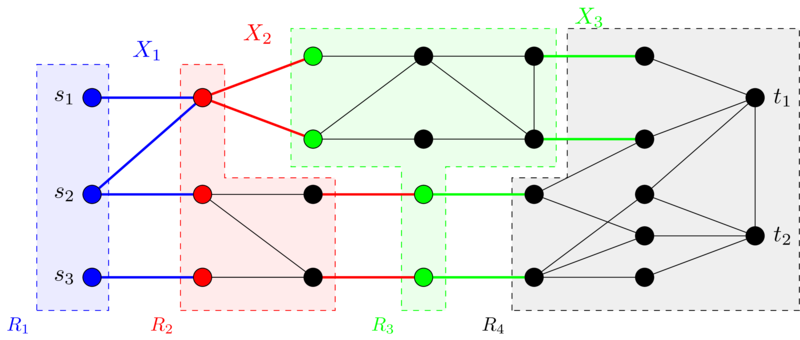
\includegraphics[width=0.8\linewidth]{etages}
\captionof{figure}{\captioncolor Décomposition en graphe à étages}
\end{center}\vspace{1cm}
  
  \item On oriente partiellement le graphe en calculant un ensemble maximum de chemins \textit{edge-disjoints}, qui ont une propriété fondamentale : \textbf{le cardinal de cet ensemble maximum est égal à la taille de la \textit{mincut}, et chaque chemin passe une et une seule fois par chaque \textit{mincut}}
  
    \begin{center}\vspace{1cm}
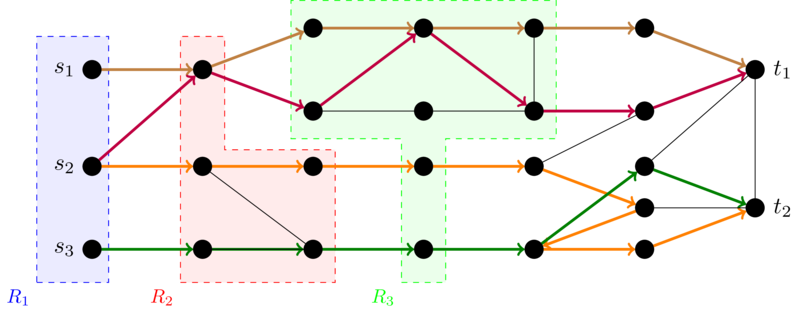
\includegraphics[width=0.8\linewidth]{mengers}
\captionof{figure}{\captioncolor Orientation du graphe selon les quatre chemins \textit{edge-disjoints}}
\end{center}\vspace{1cm}

  \item Chaque \textit{mincut} $X$ peut alors être partitionnée en $X = B \cup C$ de sorte que
  \begin{itemize}
    \item Il existe $i$ tel que $B \subseteq X_i$, et $B$ contient les arêtes de $X$ les plus à gauche
    \item Si on supprimait $X_i \backslash B$ du graphe, toutes les arêtes de $C$ seraient inaccessibles depuis $S$ dans le graphe orienté
  \end{itemize} 
  
  \item Avec cette propriété et de la combinatoire, on peut compter toutes les \textit{mincuts}
\end{enumerate}


À titre indicatif, \textbf{on obtient une complexité en $2^{O(p^2)}n^{O(1)}$}; c'est-à-dire qu'à $p$ constant, la complexité est un polynôme de $n$ multiplié par une constante exponentielle en $p^2$.

%----------------------------------------------------------------------------------------
%	PERSPECTIVES
%----------------------------------------------------------------------------------------

\color{NavyBlue} 

\section*{Perspectives}

\begin{itemize}
  \item \color{Red} Une publication pour Symposium on Theoretical Aspects of Computer Science (STACS 2019, une conférence internationale de rank A) en préparation : P. Bergé, B. Mouscadet, A. Rimmel, J. Tomasik, \textit{Fixed-parameter tractability of counting small minimum $(S,T)$-cuts}
  \color{NavyBlue} 
  \item Bien que la complexité obtenue reste grande, elle prouve que le problème est FPT, et ouvre la voie à des recherches en vue de trouver un algorithme plus optimisé 
  \item Au delà de l'aspect purement intellectuel, la résolution de ce problème a des implications dans le domaine du traitement de l'image notamment
\end{itemize}
\color{Black}
\end{multicols}
\end{document}
